%----------------------------------------------------------------------------------------
%	PART
%----------------------------------------------------------------------------------------

\part{An Introduction to Assemblers}

%----------------------------------------------------------------------------------------
%	CHAPTER
%----------------------------------------------------------------------------------------

\chapterimage{chapter_head_2} % Chapter heading image

\chapter{Assembler, Loaders and Compilers}

\textbf{An assembler translates a machine oriented language into machine language.} Machine oriented languages are more commonly known as assembly language. They are typically structured as one to one mappings to processor op codes (as we have seen earlier). However, assembly languages  also involve constructs (like psuedo instructions), macros and labels, all of which aid the programmers in writing programs and are not typically a one to one mapping to op codes.

\section{Compilers vs Assemblers}

In contrast to compilers, which are translators of languages which are machine independent in nature (have no direct mapping of instructions), assemblers are linked intrinsically to the architecture of the machine.

Architectural features such as memory word size, number formats, internal character codes, index registers, and general purpose registers, affect the way assembler instructions are written and the way the assembler handles instructions and directives. Such features are not taken in account by the compiler for higher level languages as they are built with architect agnostic features in mind.

\section{What are Loaders then ?}

Early systems had no concept of loading and linking executable and libraries. One only needed to assemble the program which would be directly loaded into the memory and run (as we saw previously in our processor simulator design). However, it was very easily seen that this cannot be a scalable model for execution. Many programs used certain sets of routines very frequently and it made no sense to write these routines every time one needed to write a program. A \textit{library} of such routines were developed along with methods to \textit{link} these routines to user code.
\textbf{Locating, loading, and linking of, assembling a single working program from individual pieces created the first assembler.}

Assemblers normally work in a two phase manner, they create a translated file from the input source known as \textbf{object file}. A loader then performs the loading, relocating, linking and starting the program from the object files (user object files, routine library files, etc).

\section{Relocation}

A program is assembled, the assembler does not know whether this is a complete program or part of a larger program. It assumes that the program will start at address zero and assembles it based on that assumption. Before the loader loads the program, it determines its true start address, based on the memory areas available at that moment and on the previously loaded object files. The loader then loads the program, making sure that all instructions fit properly in their memory locations. This process involves adjusting memory addresses in the program, and is called relocation.

\section{Benefits of Assembler Loader System}
Some of the benefits of such a system are as follows,

\begin{enumerate}
\item It makes it possible to write programs in separate parts that may also be in
different languages. Also, writing in separate parts leads in fewer bugs and higher readability.
\item When a change is made in the source code, only the modified program needs to
be reassembled. (Think of \textit{makefile})
\item The loader automatically loads routines from a standard library.
\end{enumerate}

\section{Bootstrapping}

One of the biggest questions that arises is, if you write an assembler in assembly language, how are you going to assemble it in the first place ?

This problem is solved by bootstrapping. What engineering do is that they write a very primitive assembler by hand, through manipulating op codes and then use that assembler to iteratively create a better assembler. Another method could be using a different system to write a software which cross assembles your assembler, but it's not very widely used.


%----------------------------------------------------------------------------------------
%	CHAPTER
%----------------------------------------------------------------------------------------

\chapter{Assembler Construction}

The input to any assembler is the source file. We would be talking about assemblers with respect to the assembly language that we have learned earlier. For our assembly language, each line consists of either certain instruction, a value for the previous instruction or a label.

\begin{lstlisting}[caption = Assembly Code Snippet]
movi r1
220
label: movs r1
load r2
\end{lstlisting}

In assembly languages used in industrial settings, normally there is a provision for comments and macros among other features (Assembly in such settings feels more like low-level C). We'll restrict our discussion to our bare-bones language for brevity. We will adopting a direct assemble-load model 
and wouldn't be discussing much about loaders.

\begin{figure}
\caption{A Typical Assembler}
\label{fig:assmblr}
\centering
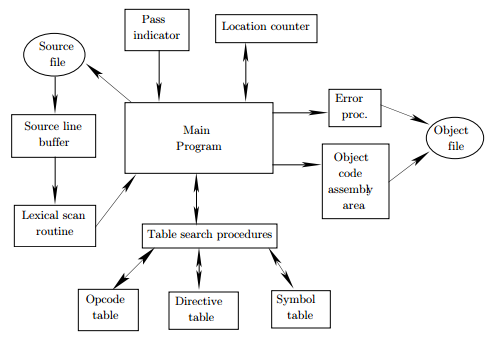
\includegraphics[width=0.4\textwidth]{assembler_block}
\end{figure}

\section{Deconstructing the Source File}

\subsection{Instructions}

The instructions normally are identified by the mnemonic and are directly mapped to some op code of the processor. The assembler is the one which defines this mapping through a table. It also keeps a track of structure of the intruction, ie. number of operands. 

Instructions can have zero, one, or two operands (some processors also have three operand instructions). The operands supply information to the assembler about the source line.
For example, \textit{movi} has 2 operands, the register in which we want to move and the value to be stored in it.

\subsection{Labels and References}

The label is necessary if we want to refer the instruction from some other point in the program. Now, where we refer to this label leads to two kind of references, "forward references" and "backward references". Forward References are those references where you refer to label that hasn't been defined yet (future label), if you read line by line from start. 

\begin{lstlisting}[caption = Forward Reference in Assembly]
jmpdnz
label
..
..
label: movs r1
load r2
\end{lstlisting}

Backward References are the ones that have been defined already. Obviously, future labels are not an error and their use should not be prohibited. The programmer should be able to refer to source lines which either precede or follow the current line. The problem of handling references is the core issue while writing Assemblers.

\section{Important Elements}

\subsection{OpCode Table}

To translate an instruction, the assembler uses the OpCode table, which is a static data structure. The two important columns in the table are the mnemonic and OpCode.

The OpCode table should be good for searching instructions. For each source line input, the assembler has to search the OpCode table. If it finds the mnemonic, it uses the OpCode to start assembling the instruction. It also uses the other information in the OpCode table, like number of operands etc to complete the assembly.

This table can be implemented in various ways, most notably using a hash table, which you will study in Data Structures if you haven't already.

\subsection{Symbol Table}

The symbol table is dynamic table that is used by the assembler, initially empty. Each entry in the table contains the definition of a label and stores the position of the label. Labels are added as they are encountered in the source file, and the table is also searched frequently to find the values of known labels, which is basically a reference to instruction number.

\newpage

\section{Two-Pass Assembler}

\begin{figure}[h]
\caption{A Typical Two Pass Assembler}
\label{fig:twopass}
\centering
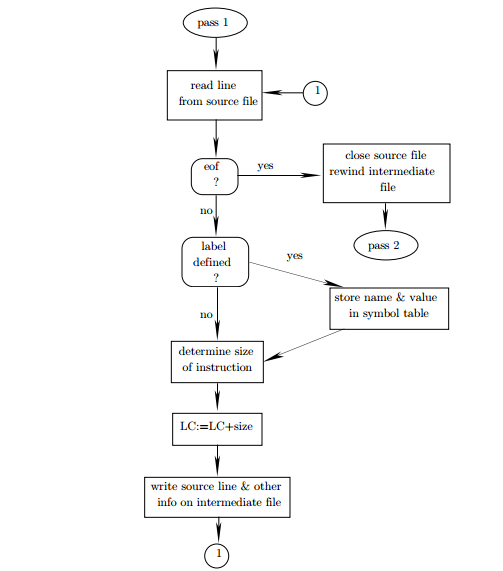
\includegraphics[width=0.6\textwidth]{two_pass_algo}
\end{figure}

A two-pass assembler is easier to understand and will be discussed first. Such
an assembler performs two passes over the source file. In the first pass it reads the
entire source file, looking only for label definitions. All labels are collected, assigned
values, and placed in the symbol table in this pass. No instructions are assembled
and, at the end of the pass, the symbol table should contain all the labels defined in
the program. In the second pass, the instructions are again read and are assembled,
using the symbol table. An assembler in our keeps
the size of each instruction in the OpCode table together with the mnemonic and
the OpCode
